\documentclass[12pt,a4paper]{article}

% ─── Page Layout ───────────────────────────────────────────────────────────────
\usepackage[a4paper, margin=0.8in, headheight=14pt]{geometry}

% ─── Fonts (XeLaTeX) ───────────────────────────────────────────────────────────
\usepackage{fontspec}
\usepackage{unicode-math}
\setmainfont{TeX Gyre Pagella}
\setmonofont[Scale=0.88]{TeX Gyre Cursor}
\setmathfont{Latin Modern Math}

% ─── Packages ──────────────────────────────────────────────────────────────────
\usepackage{xcolor}
\usepackage{colortbl}
\usepackage{titlesec}
\usepackage{enumitem}
\usepackage{tabularx}
\usepackage{booktabs}
\usepackage{array}
\usepackage{amsmath}
\usepackage{tikz}
\usetikzlibrary{shapes.geometric, arrows.meta, positioning, calc, fit, decorations.pathreplacing}
\usepackage{tcolorbox}
\tcbuselibrary{skins, breakable}
\usepackage{hyperref}
\usepackage{fancyhdr}
\usepackage{graphicx}
\usepackage{microtype}
\hyphenpenalty=10000
\exhyphenpenalty=10000
\sloppy
\usepackage{caption}
\usepackage{setspace}
\usepackage{multirow}
\usepackage{tocloft}

% ─── Q&A helper ────────────────────────────────────────────────────────────────
\newcommand{\Q}[1]{\textbf{#1}\par\noindent\ignorespaces}

% ─── Colour Palette ────────────────────────────────────────────────────────────
\definecolor{myred}{RGB}{196,30,58}
\definecolor{mydark}{RGB}{30,30,50}
\definecolor{mygreen}{RGB}{14,120,80}
\definecolor{myteal}{RGB}{0,130,140}
\definecolor{myamber}{RGB}{180,100,0}
\definecolor{mypurple}{RGB}{100,30,160}
\definecolor{mygray}{RGB}{246,247,249}
\definecolor{mgframe}{RGB}{180,185,200}
\definecolor{watermark}{RGB}{145,150,170}
\definecolor{hdrred}{RGB}{250,232,235}
\definecolor{hdrgreen}{RGB}{220,244,233}
\definecolor{hdrteal}{RGB}{220,242,244}
\definecolor{hdramber}{RGB}{253,242,215}
\definecolor{hdrpurple}{RGB}{238,228,255}
\definecolor{hdrgray}{RGB}{238,240,245}
\definecolor{rowalt}{RGB}{250,251,253}

% ─── Section Formatting ────────────────────────────────────────────────────────
\titleformat{\section}
  {\large\bfseries\color{myred}}{\thesection.}{0.5em}{}
  [\vspace{1pt}{\color{myred}\rule{\linewidth}{0.8pt}}]
\titleformat{\subsection}
  {\normalsize\bfseries\color{myteal}}{\thesubsection}{0.5em}{}
\titlespacing*{\section}{0pt}{18pt}{7pt}
\titlespacing*{\subsection}{0pt}{11pt}{4pt}

% ─── Paragraph ─────────────────────────────────────────────────────────────────
\setlength{\parindent}{0pt}
\setlength{\parskip}{4pt}

% ─── TOC Styling ───────────────────────────────────────────────────────────────
\renewcommand{\cfttoctitlefont}{\large\bfseries\color{myred}}
\renewcommand{\cftaftertoctitle}{\par\noindent{\color{myred}\rule{\linewidth}{0.8pt}}}
\setlength{\cftbeforetoctitleskip}{0pt}
\setlength{\cftaftertoctitleskip}{6pt}
\renewcommand{\cftsecfont}{\normalsize\bfseries\color{mydark}}
\renewcommand{\cftsecpagefont}{\normalsize\bfseries\color{mydark}}
\renewcommand{\cftsecleader}{\cftdotfill{\cftdotsep}}
\setlength{\cftbeforesecskip}{7pt}
\renewcommand{\cftsubsecfont}{\small\color{mydark}}
\renewcommand{\cftsubsecpagefont}{\small\color{mydark}}
\setlength{\cftbeforesubsecskip}{3pt}
\setlength{\cftsubsecindent}{1.4em}

% ─── Table helpers ─────────────────────────────────────────────────────────────
\renewcommand{\arraystretch}{1.45}
\setlength{\tabcolsep}{6pt}
\arrayrulecolor{mydark}
\newcolumntype{B}[1]{>{\small\bfseries\raggedright\arraybackslash}m{#1}}
\newcolumntype{Y}{>{\small\raggedright\arraybackslash}X}
\renewcommand{\tabularxcolumn}[1]{m{#1}}

% ─── Header / Footer ───────────────────────────────────────────────────────────
\pagestyle{fancy}
\fancyhf{}
\fancyhead[L]{\small\color{myred}\textbf{HS-HU701}\;\color{mydark}--- Principles of Management}
\fancyhead[R]{\small\color{myteal}\textbf{Module 2 Notes}}
\fancyfoot[C]{\small\color{mydark}\thepage}
\fancyfoot[R]{\small\color{watermark}\textit{\copyright\ Biraj}}
\renewcommand{\headrulewidth}{0.5pt}
\renewcommand{\footrulewidth}{0.3pt}

% ─── Hyperref ──────────────────────────────────────────────────────────────────
\hypersetup{
  colorlinks=true, linkcolor=myteal, urlcolor=myteal,
  pdfauthor={Biraj Sarkar},
  pdftitle={HS-HU701 --- Module 2 Notes}
}

% ─── tcolorbox styles ──────────────────────────────────────────────────────────
\tcbset{
  tikzbox/.style={
    colback=mygray, colframe=mgframe, boxrule=0.6pt, arc=4pt,
    left=8pt, right=8pt, top=6pt, bottom=6pt,
    colbacktitle=mgframe, coltitle=mydark,
    fonttitle=\small\bfseries
  },
  defbox/.style={
    colback=hdrgreen, colframe=mygreen, boxrule=0.8pt, arc=4pt,
    left=9pt, right=9pt, top=6pt, bottom=6pt,
    colbacktitle=mygreen, coltitle=white,
    fonttitle=\small\bfseries
  },
  formulabox/.style={
    colback=hdrteal, colframe=myteal, boxrule=0.8pt, arc=4pt,
    left=9pt, right=9pt, top=7pt, bottom=7pt,
    colbacktitle=myteal, coltitle=white,
    fonttitle=\small\bfseries
  },
  examplebox/.style={
    colback=hdramber, colframe=myamber, boxrule=0.8pt, arc=4pt,
    left=9pt, right=9pt, top=6pt, bottom=6pt,
    colbacktitle=myamber, coltitle=white,
    fonttitle=\small\bfseries
  },
  masonbox/.style={
    colback=hdrpurple, colframe=mypurple, boxrule=0.8pt, arc=4pt,
    left=9pt, right=9pt, top=6pt, bottom=6pt,
    colbacktitle=mypurple, coltitle=white,
    fonttitle=\small\bfseries
  },
  exambox/.style={
    colback=hdrpurple, colframe=mypurple, boxrule=1pt, arc=5pt,
    left=10pt, right=10pt, top=8pt, bottom=8pt,
    colbacktitle=mypurple, coltitle=white,
    fonttitle=\bfseries,
    breakable, title after break={\textbf{Frequently Asked / Viva Questions (contd.)}}}
}
\tcbset{breakable}

% ─── TikZ styles ───────────────────────────────────────────────────────────────
\tikzset{
  block/.style={rectangle, draw=myteal, fill=hdrteal,
    text width=2.4cm, align=center, minimum height=0.95cm,
    font=\small, rounded corners=3pt, line width=0.7pt},
  redblock/.style={rectangle, draw=myred, fill=hdrred,
    text width=2.4cm, align=center, minimum height=0.95cm,
    font=\small, rounded corners=3pt, line width=0.7pt},
  netnode/.style={rectangle, draw=myteal, fill=hdrteal,
    text width=1.5cm, align=center, minimum height=0.8cm,
    font=\small, rounded corners=3pt, line width=0.7pt},
  sumjunc/.style={circle, draw=myamber, fill=hdramber,
    minimum size=0.62cm, font=\small, line width=0.8pt},
  snode/.style={circle, draw=mypurple, fill=hdrpurple,
    minimum size=0.55cm, font=\footnotesize, line width=0.7pt},
  arrow/.style={-Stealth, thick, color=mydark},
  redarrow/.style={-Stealth, thick, color=myred},
  line/.style={thick, color=mydark}
}

% ═══════════════════════════════════════════════════════════════════════════════
\begin{document}
% ═══════════════════════════════════════════════════════════════════════════════

\begin{center}
  {\LARGE\bfseries\color{myred} HS-HU701 --- Principles of Management}\\[5pt]
  {\normalsize\color{mydark} Semester VII \quad$\bullet$\quad 2L:0T:0P \quad$\bullet$\quad 2 Credits}\\[3pt]
  {\normalsize\color{myteal}\textbf{Module 2 Exam Notes}}\\[3pt]
  {\small\color{mydark} CGEC \;$|$\; B.Tech ECE (2023--27) \;$|$\; \textit{Biraj Sarkar}}
\end{center}
\vspace{2pt}
\noindent{\color{myred}\rule{\linewidth}{1.5pt}}
\vspace{2pt}

\hypersetup{linkcolor=mydark}
\tableofcontents
\hypersetup{linkcolor=myteal}
\newpage

% ===============================================================================
\section{Management and Society}
% ===============================================================================

\begin{tcolorbox}[defbox, title={\textbf{Management and Society --- Overview}}]
\textbf{Management and Society} refers to the interdependent relationship between organisations and their social environment. Modern organisations are not isolated entities; they are open systems embedded within society and are affected by social, political, legal, and economic forces --- and, in turn, they affect society.
\end{tcolorbox}

\subsection{External Environment of an Organisation}
The external environment consists of all forces outside the organisation that can influence its performance:

\begin{tcolorbox}[tikzbox, title={External Environment of an Organisation}]
\centering
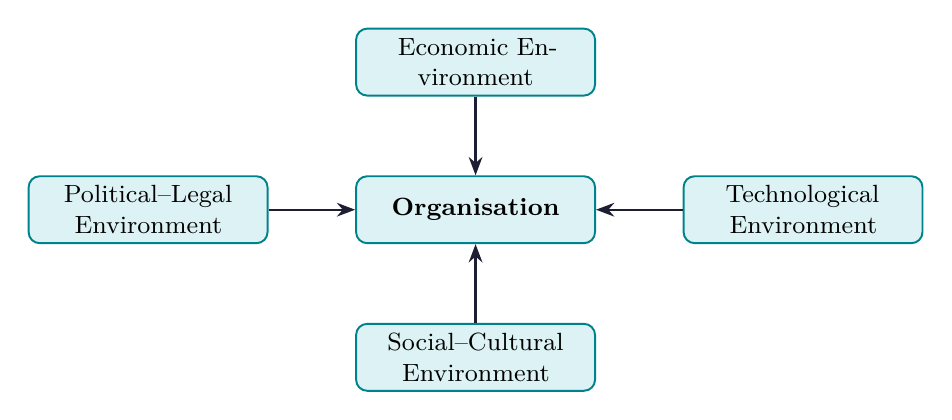
\begin{tikzpicture}[
  envbox/.style={rectangle, draw=myteal, fill=hdrteal, text width=2.8cm,
    align=center, minimum height=0.85cm, font=\small, rounded corners=4pt, line width=0.7pt},
  arrow/.style={-Stealth, thick, color=mydark}
]
  \node[envbox] (org) at (0,0) {\textbf{Organisation}};
  \node[envbox, above=1.0cm of org] (eco) {Economic Environment};
  \node[envbox, right=1.1cm of org] (tech) {Technological Environment};
  \node[envbox, below=1.0cm of org] (soc) {Social--Cultural Environment};
  \node[envbox, left=1.1cm of org] (pol) {Political--Legal Environment};

  \draw[arrow] (eco) -- (org);
  \draw[arrow] (tech) -- (org);
  \draw[arrow] (soc) -- (org);
  \draw[arrow] (pol) -- (org);
\end{tikzpicture}
\end{tcolorbox}

\begin{itemize}[leftmargin=*, itemsep=3pt]
  \item \textbf{Economic Environment:} Includes inflation, interest rates, GDP growth, unemployment levels, and business cycles. Directly affects demand, costs, and investment decisions.
  \item \textbf{Technological Environment:} Pace of innovation, automation, R\&D, and digitisation. Affects production methods, products, and competitive advantage.
  \item \textbf{Social--Cultural Environment:} Demographics, lifestyle changes, cultural values, education levels, and social norms. Affects consumer behaviour and workforce composition.
  \item \textbf{Political--Legal Environment:} Government stability, taxation policy, labour laws, environmental regulations, and trade policies. Shapes the rules within which organisations operate.
  \item \textbf{Natural Environment:} Availability of natural resources, environmental sustainability concerns, climate regulations.
\end{itemize}

\subsection{Corporate Social Responsibility (CSR)}

\begin{tcolorbox}[defbox, title={\textbf{Corporate Social Responsibility (CSR)}}]
\textbf{CSR} is the obligation of business organisations to act in ways that protect and improve the welfare of society along with their own interests. It represents a company's commitment to operating in an economically, socially, and environmentally responsible manner beyond what the law requires.
\end{tcolorbox}

\subsubsection{Carroll's Pyramid of CSR}
Carroll (1991) proposed four layers of corporate responsibility, from the most fundamental to the most discretionary:

\begin{tcolorbox}[tikzbox, title={Carroll's Pyramid of CSR}]
\centering
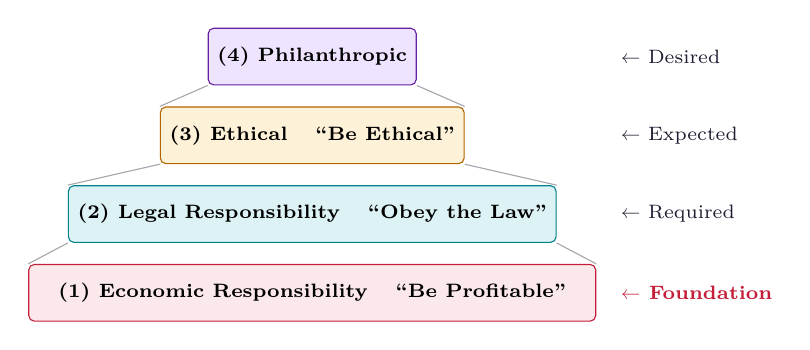
\begin{tikzpicture}[every node/.style={align=center}]
  % Pyramid layers — bottom (widest) to top (narrowest), centered at x=0
  % Each layer: box on left, label on right (with enough offset)
  \node[draw=myred, fill=hdrred, minimum width=7.2cm, minimum height=0.72cm,
    font=\scriptsize\bfseries, rounded corners=2pt] (eco) at (0, 0)
    {(1) Economic Responsibility \quad ``Be Profitable''};

  \node[draw=myteal, fill=hdrteal, minimum width=5.4cm, minimum height=0.72cm,
    font=\scriptsize\bfseries, rounded corners=2pt] (leg) at (0, 1.0)
    {(2) Legal Responsibility \quad ``Obey the Law''};

  \node[draw=myamber, fill=hdramber, minimum width=3.6cm, minimum height=0.72cm,
    font=\scriptsize\bfseries, rounded corners=2pt] (eth) at (0, 2.0)
    {(3) Ethical \quad ``Be Ethical''};

  \node[draw=mypurple, fill=hdrpurple, minimum width=1.8cm, minimum height=0.72cm,
    font=\scriptsize\bfseries, rounded corners=2pt] (phi) at (0, 3.0)
    {(4) Philanthropic};

  % Right-side labels placed well clear of the boxes
  \node[font=\scriptsize\bfseries\color{myred},   anchor=west] at (3.8, 0)   {$\leftarrow$ Foundation};
  \node[font=\scriptsize\color{mydark},            anchor=west] at (3.8, 1.0) {$\leftarrow$ Required};
  \node[font=\scriptsize\color{mydark},            anchor=west] at (3.8, 2.0) {$\leftarrow$ Expected};
  \node[font=\scriptsize\color{mydark},            anchor=west] at (3.8, 3.0) {$\leftarrow$ Desired};

  % Connecting lines between layers to show pyramid structure
  \draw[mydark!40, thin] (eco.north west) -- (leg.south west);
  \draw[mydark!40, thin] (eco.north east) -- (leg.south east);
  \draw[mydark!40, thin] (leg.north west) -- (eth.south west);
  \draw[mydark!40, thin] (leg.north east) -- (eth.south east);
  \draw[mydark!40, thin] (eth.north west) -- (phi.south west);
  \draw[mydark!40, thin] (eth.north east) -- (phi.south east);
\end{tikzpicture}
\end{tcolorbox}

\subsubsection{Arguments For and Against CSR}
\par\noindent
{\renewcommand{\arraystretch}{1.55}%
\begin{tabularx}{\linewidth}{|Y|Y|}\hline
\multicolumn{1}{|>{\centering\arraybackslash}Y|}{\textbf{Arguments For CSR}} &
\multicolumn{1}{>{\centering\arraybackslash}Y|}{\textbf{Arguments Against CSR}} \\[4pt]
\hline
Improves brand image and public trust. & Increases costs and reduces profitability. \\
\hline
Attracts socially conscious investors and customers. & Management's primary duty is profit maximisation (Friedman doctrine). \\[4pt]
\hline
Reduces regulatory scrutiny and legal risk. & Dilutes focus from core business competence. \\
\hline
Enhances employee motivation and retention. & Can lead to misuse of corporate funds. \\
\hline
Contributes to long-term sustainable development. & Difficult to measure the return on CSR investment. \\[4pt]
\hline
\end{tabularx}
}

\subsection{Corporate Governance}

\begin{tcolorbox}[defbox, title={\textbf{Corporate Governance}}]
\textbf{Corporate Governance} refers to the system of rules, practices, and processes by which a company is directed and controlled. It balances the interests of a company's many stakeholders --- shareholders, management, customers, suppliers, financiers, government, and the community.
\end{tcolorbox}

\textbf{Key principles of Good Corporate Governance:}
\begin{itemize}[leftmargin=*, itemsep=2pt]
  \item \textbf{Accountability:} Directors and management are accountable to shareholders.
  \item \textbf{Transparency:} Full, accurate, and timely disclosure of financial and non-financial information.
  \item \textbf{Fairness:} Equal treatment of all shareholders, including minority shareholders.
  \item \textbf{Responsibility:} Management must act responsibly toward all stakeholders.
  \item \textbf{Independence:} Independent board members free from management influence.
\end{itemize}

\subsection{Ethical Standards in Management}

\begin{tcolorbox}[defbox, title={\textbf{Business Ethics}}]
\textbf{Business Ethics} refers to the application of ethical principles and moral standards to business activities, relationships, and decisions. It involves distinguishing between right and wrong conduct in the workplace.
\end{tcolorbox}

\textbf{Sources of unethical behaviour in organisations:}
\begin{itemize}[leftmargin=*, itemsep=2pt]
  \item Excessive pressure to meet short-term financial targets.
  \item Ambiguous or absent codes of conduct.
  \item Weak enforcement of ethical standards by top management.
  \item Peer pressure and cultural normalisation of unethical acts.
\end{itemize}

\textbf{How to improve ethical standards:}
\begin{itemize}[leftmargin=*, itemsep=2pt]
  \item Develop and communicate a formal Code of Ethics.
  \item Lead by example --- ethical behaviour from top management.
  \item Establish whistleblower protection mechanisms.
  \item Conduct regular ethics training programmes.
  \item Include ethical criteria in performance appraisal.
\end{itemize}

% ===============================================================================
\section{People Management}
% ===============================================================================

\begin{tcolorbox}[defbox, title={\textbf{People Management --- Overview}}]
\textbf{People Management} (Human Resource Management) involves planning for, acquiring, developing, and retaining people in an organisation so that they contribute maximally to organisational goals.
\end{tcolorbox}

\subsection{Job Design}

\begin{tcolorbox}[defbox, title={\textbf{Job Design}}]
\textbf{Job Design} is the process of organising tasks, duties, and responsibilities into a productive unit of work. It defines the content and method of a job and influences employee motivation, satisfaction, and productivity.
\end{tcolorbox}

\textbf{Major approaches to job design:}
\begin{enumerate}[label=\textbf{\arabic*.}, leftmargin=*, itemsep=3pt, topsep=2pt]
  \item \textbf{Job Simplification:} Breaking jobs into small, repetitive, standardised tasks. Maximises efficiency but may cause boredom (Taylor's Scientific Management approach).
  \item \textbf{Job Rotation:} Systematically moving employees across different jobs or departments. Reduces boredom and builds versatility.
  \item \textbf{Job Enlargement:} Adding more tasks of similar complexity to a job (horizontal expansion) to increase variety.
  \item \textbf{Job Enrichment:} Adding more responsibility, autonomy, and complexity to a job (vertical expansion). Based on Herzberg's two-factor theory --- enhances motivation.
\end{enumerate}

\textbf{Hackman and Oldham's Job Characteristics Model} identifies five core dimensions:
\begin{itemize}[leftmargin=*, itemsep=2pt]
  \item \textbf{Skill variety:} Degree to which a job requires different skills and talents.
  \item \textbf{Task identity:} Degree to which the job involves doing a complete piece of work.
  \item \textbf{Task significance:} Degree to which the job has a substantial impact on others.
  \item \textbf{Autonomy:} Degree to which the job provides freedom and independence.
  \item \textbf{Feedback:} Degree to which the job itself provides direct performance information.
\end{itemize}

\subsection{Recruitment and Selection}

\begin{tcolorbox}[defbox, title={\textbf{Recruitment and Selection}}]
\textbf{Recruitment} is the process of attracting qualified candidates for job vacancies. \textbf{Selection} is the process of choosing the most suitable candidate from the pool of recruited applicants.
\end{tcolorbox}

\par\noindent
{\renewcommand{\arraystretch}{1.55}%
\begin{tabularx}{\linewidth}{|B{3.0cm}|Y|Y|}\hline
\multicolumn{1}{|>{\centering\arraybackslash}m{3.0cm}|}{\textbf{Aspect}} &
\multicolumn{1}{>{\centering\arraybackslash}Y|}{\textbf{Recruitment}} &
\multicolumn{1}{>{\centering\arraybackslash}Y|}{\textbf{Selection}} \\[4pt]
\hline
Definition & Attracting a pool of qualified applicants. & Choosing the best fit from the applicants. \\[4pt]
\hline
Nature & Positive process (attract more applicants). & Negative process (eliminate unsuitable candidates). \\[4pt]
\hline
Outcome & Pool of candidates. & Single best candidate appointed. \\
\hline
Sources & Internal (promotions, transfers) or External (ads, job fairs, campus). & Interviews, tests, background checks. \\[4pt]
\hline
\end{tabularx}
}

\subsection{Training and Development}

\begin{tcolorbox}[defbox, title={\textbf{Training vs.\ Development}}]
\textbf{Training} is a short-term, systematic process that improves employees' specific job-related skills and knowledge for their current role.
\par\vspace{3pt}
\textbf{Development} is a long-term process aimed at improving the overall capabilities and career growth of employees for future roles.
\end{tcolorbox}

\textbf{Common training methods:}
\begin{itemize}[leftmargin=*, itemsep=2pt]
  \item \textbf{On-the-Job Training (OJT):} Apprenticeship, coaching, mentoring, job rotation.
  \item \textbf{Off-the-Job Training:} Lectures, case studies, simulations, vestibule training, role-playing.
  \item \textbf{E-Learning:} Online courses, virtual classrooms, webinars.
\end{itemize}

\subsection{Stress Management}

\begin{tcolorbox}[defbox, title={\textbf{Stress in the Workplace}}]
\textbf{Stress} is the physical and emotional response to excessive demands or pressures that exceed a person's ability to cope. Moderate stress (eustress) can improve performance, but chronic stress (distress) reduces productivity and health.
\end{tcolorbox}

\textbf{Common causes of workplace stress (stressors):}
\begin{itemize}[leftmargin=*, itemsep=2pt]
  \item Work overload, unrealistic deadlines, and poor time management.
  \item Role ambiguity (unclear responsibilities) or role conflict (conflicting demands).
  \item Poor relationships with supervisors or colleagues.
  \item Job insecurity and lack of career growth opportunities.
  \item Physical conditions: noise, poor lighting, and uncomfortable workspace.
\end{itemize}

\textbf{Stress management strategies:}
\par\noindent
{\renewcommand{\arraystretch}{1.55}%
\begin{tabularx}{\linewidth}{|B{3.2cm}|Y|}\hline
\multicolumn{1}{|>{\centering\arraybackslash}m{3.2cm}|}{\textbf{Approach}} &
\multicolumn{1}{>{\centering\arraybackslash}Y|}{\textbf{Methods}} \\[4pt]
\hline
Individual (employee) & Time management, exercise, relaxation techniques, social support. \\
\hline
Organisational & Clear role definitions, flexible work arrangements, counselling programmes, realistic goal-setting. \\[4pt]
\hline
Job Redesign & Reducing overload; increasing autonomy and feedback. \\
\hline
\end{tabularx}
}

% ===============================================================================
\section{Managerial Competencies}
% ===============================================================================

\subsection{Communication in Management}

\begin{tcolorbox}[defbox, title={\textbf{Communication --- Definition}}]
\textbf{Communication} is the process of transmitting information, ideas, thoughts, feelings, and emotions from one person to another through verbal, non-verbal, or written channels. Effective communication is essential for coordination, motivation, and decision-making.
\end{tcolorbox}

\textbf{Types of communication in an organisation:}
\begin{itemize}[leftmargin=*, itemsep=2pt]
  \item \textbf{Downward:} From higher to lower levels (orders, policies, instructions).
  \item \textbf{Upward:} From lower to higher levels (reports, feedback, grievances).
  \item \textbf{Horizontal/Lateral:} Among peers at the same level (coordination).
  \item \textbf{Diagonal:} Across different levels and departments (cross-functional teams).
  \item \textbf{Grapevine (Informal):} Unofficial communication networks; fast but often inaccurate.
\end{itemize}

\textbf{Barriers to effective communication:}
\begin{itemize}[leftmargin=*, itemsep=2pt]
  \item Physical barriers (noise, distance), Semantic barriers (jargon, language differences).
  \item Psychological barriers (perceptual biases, emotional state).
  \item Organisational barriers (rigid hierarchies, information overload).
\end{itemize}

\subsection{Motivation}

\begin{tcolorbox}[defbox, title={\textbf{Motivation --- Definition}}]
\textbf{Motivation} is the process that initiates, guides, and sustains goal-oriented behaviours. It is the internal force that drives an individual to take action, maintain effort, and persist toward a goal.
\end{tcolorbox}

\textbf{Major motivation theories:}

\par\noindent
{\renewcommand{\arraystretch}{1.55}%
\begin{tabularx}{\linewidth}{|B{3.5cm}|Y|}\hline
\multicolumn{1}{|>{\centering\arraybackslash}m{3.5cm}|}{\textbf{Theory}} &
\multicolumn{1}{>{\centering\arraybackslash}Y|}{\textbf{Key Concept}} \\[4pt]
\hline
Maslow's Hierarchy of Needs & Five levels: Physiological $\to$ Safety $\to$ Social $\to$ Esteem $\to$ Self-Actualisation. People are motivated to fulfil unmet needs. \\[4pt]
\hline
Herzberg's Two-Factor Theory & \textbf{Hygiene factors} (salary, job security) prevent dissatisfaction. \textbf{Motivators} (achievement, recognition) create satisfaction. \\[4pt]
\hline
McGregor's Theory X and Y & Theory X: Workers are lazy and need control. Theory Y: Workers are self-motivated and seek responsibility. \\[4pt]
\hline
Vroom's Expectancy Theory & Motivation $=$ Expectancy $\times$ Instrumentality $\times$ Valence. Effort leads to performance, performance leads to outcome. \\[4pt]
\hline
\end{tabularx}
}

\subsection{Team Effectiveness}

\begin{tcolorbox}[defbox, title={\textbf{Team vs.\ Group}}]
A \textbf{Group} is a collection of individuals who interact primarily to share information and make decisions. A \textbf{Team} is a small number of people with complementary skills who are committed to a common purpose, performance goals, and approach for which they hold themselves mutually accountable.
\end{tcolorbox}

\textbf{Tuckman's Stages of Team Development:}
\begin{enumerate}[label=\textbf{\arabic*.}, leftmargin=*, itemsep=2pt, topsep=2pt]
  \item \textbf{Forming:} Team members are introduced; roles and goals are unclear; polite and cautious behaviour.
  \item \textbf{Storming:} Conflict and competition arise as individual personalities emerge; power struggles.
  \item \textbf{Norming:} Team establishes norms, roles become clear, cohesion builds.
  \item \textbf{Performing:} Team works productively and cooperatively toward goals.
  \item \textbf{Adjourning:} Team disbands after goal achievement; members reflect on accomplishments.
\end{enumerate}

\subsection{Conflict Management}

\begin{tcolorbox}[defbox, title={\textbf{Conflict in Organisations}}]
\textbf{Conflict} is a disagreement between two or more parties over incompatible goals, limited resources, or differences in values and perceptions. Conflict can be \textbf{functional} (stimulates creativity and debate) or \textbf{dysfunctional} (destroys cohesion and performance).
\end{tcolorbox}

\textbf{Thomas--Kilmann Conflict Resolution Styles:}
\par\noindent
{\renewcommand{\arraystretch}{1.55}%
\begin{tabularx}{\linewidth}{|B{2.8cm}|Y|Y|}\hline
\multicolumn{1}{|>{\centering\arraybackslash}m{2.8cm}|}{\textbf{Style}} &
\multicolumn{1}{>{\centering\arraybackslash}Y|}{\textbf{Description}} &
\multicolumn{1}{>{\centering\arraybackslash}Y|}{\textbf{When to Use}} \\[4pt]
\hline
Competing & Assert own position; win--lose approach. & Emergencies; unpopular decisions. \\
\hline
Collaborating & Win--win; both parties work together to find a mutually satisfying solution. & Complex issues; long-term relationships. \\[4pt]
\hline
Compromising & Each party gives up something; middle-ground solution. & Time pressure; equal-power parties. \\[4pt]
\hline
Avoiding & Withdraw or postpone the conflict. & Trivial issues; when time is needed to cool down. \\
\hline
Accommodating & Yield to the other party; lose--win. & When preserving relationship is more important than outcome. \\[4pt]
\hline
\end{tabularx}
}

\subsection{Creativity and Entrepreneurship}

\begin{tcolorbox}[defbox, title={\textbf{Creativity and Entrepreneurship}}]
\textbf{Creativity} is the ability to generate novel and useful ideas. \textbf{Entrepreneurship} is the process of identifying business opportunities and organising resources to exploit them, while accepting the associated risks.
\par\vspace{3pt}
\textbf{Intrapreneurship:} Entrepreneurial behaviour within an existing organisation --- employees act as internal entrepreneurs to develop new products or processes.
\end{tcolorbox}

\textbf{Characteristics of creative/entrepreneurial managers:}
\begin{itemize}[leftmargin=*, itemsep=2pt]
  \item High tolerance for ambiguity and risk.
  \item Intrinsic motivation and persistent problem-solving drive.
  \item Ability to connect disparate ideas and synthesise novel solutions.
  \item Strong networking and resource-mobilisation skills.
\end{itemize}

% ===============================================================================
% MANDATORY QUICK REVISION PAGE
% ===============================================================================
\newpage
\begin{center}
  {\large\bfseries\color{myred} Quick Revision --- Module 2}\\[3pt]
  {\small\color{mydark} Society, People Management \& Managerial Competencies $|$ HS-HU701}
\end{center}
\noindent{\color{myred}\rule{\linewidth}{1.2pt}}
\vspace{4pt}

\begin{tcolorbox}[formulabox, title={\textbf{Key Frameworks at a Glance}}]
\renewcommand{\arraystretch}{1.3}
\begin{tabularx}{\linewidth}{B{4.0cm} X}Carroll's CSR Pyramid & Economic $\to$ Legal $\to$ Ethical $\to$ Philanthropic \\[3pt]
Job Enrichment & Vertical job expansion; adds autonomy and responsibility. \\[3pt]
Vroom's Expectancy & Motivation $=$ Expectancy $\times$ Instrumentality $\times$ Valence \\[3pt]
Tuckman's Team Stages & Forming $\to$ Storming $\to$ Norming $\to$ Performing $\to$ Adjourning \\[3pt]
Thomas--Kilmann & 5 conflict styles: Competing, Collaborating, Compromising, Avoiding, Accommodating \\
\end{tabularx}
\end{tcolorbox}

\begin{tcolorbox}[defbox, title={\textbf{One-Line Definitions}}]
\begin{itemize}[leftmargin=*, itemsep=2pt, topsep=0pt]
  \item \textbf{CSR:} Obligation of organisations to operate in a socially and environmentally responsible manner beyond legal requirements.
  \item \textbf{Corporate Governance:} System of rules and processes by which a company is directed and controlled.
  \item \textbf{Business Ethics:} Application of moral standards to business activities and decisions.
  \item \textbf{Job Design:} Organising tasks and responsibilities into a productive unit of work.
  \item \textbf{Job Enrichment:} Vertical expansion of a job by adding responsibility and autonomy.
  \item \textbf{Recruitment:} Process of attracting qualified candidates for vacancies (positive process).
  \item \textbf{Selection:} Process of choosing the best fit from recruited candidates (negative/elimination process).
  \item \textbf{Stress:} Emotional/physical response when demands exceed coping capacity.
  \item \textbf{Motivation:} Internal force that drives behaviour toward a goal.
  \item \textbf{Team:} Small group with complementary skills, shared goals, and mutual accountability.
  \item \textbf{Conflict:} Disagreement over incompatible goals, resources, or values.
  \item \textbf{Entrepreneurship:} Identifying opportunities and organising resources to exploit them while accepting risk.
\end{itemize}
\end{tcolorbox}

\begin{tcolorbox}[exambox, title={\textbf{Frequently Asked / Viva Questions}}]
\begin{enumerate}[topsep=0pt, label=\textbf{Q\arabic*.}, itemsep=5pt]
  \item \Q{What is CSR? What are Carroll's four levels of CSR?}
    CSR is a firm's commitment to act ethically and contribute to economic development while improving the quality of life. Carroll's four levels are: Economic (be profitable), Legal (obey the law), Ethical (be ethical), and Philanthropic (be a good citizen).
  \item \Q{What is Corporate Governance? Why is it important?}
    Corporate governance is the system of rules directing and controlling a company. It ensures accountability, transparency, and fair treatment of all stakeholders, preventing fraud and mismanagement.
  \item \Q{Distinguish between job enrichment and job enlargement.}
    Job enrichment adds more responsibility, autonomy, and complexity (vertical expansion). Job enlargement adds more tasks of similar difficulty (horizontal expansion). Enrichment is more motivating.
  \item \Q{What is Tuckman's model of team development? Name the five stages.}
    Tuckman's model describes team evolution through: Forming (polite, uncertain), Storming (conflict), Norming (cohesion), Performing (productive), and Adjourning (disbanding).
  \item \Q{State Herzberg's Two-Factor Theory. How does it differ from Maslow's theory?}
    Herzberg identifies Hygiene Factors (prevent dissatisfaction: salary, working conditions) and Motivators (create satisfaction: achievement, recognition). Unlike Maslow's single hierarchy, Herzberg separates dissatisfaction and satisfaction as two independent dimensions.
  \item \Q{What is Vroom's Expectancy Theory of motivation?}
    Motivation = Expectancy (effort will lead to performance) $\times$ Instrumentality (performance will lead to reward) $\times$ Valence (reward is valued). All three must be high for strong motivation.
  \item \Q{What are the five Thomas--Kilmann conflict resolution styles?}
    Competing (win--lose), Collaborating (win--win), Compromising (mutual concessions), Avoiding (withdraw), and Accommodating (yield to other party).
  \item \Q{What is the difference between recruitment and selection?}
    Recruitment is a positive process of attracting a pool of candidates; selection is a negative process of eliminating unsuitable candidates to choose the best fit.
  \item \Q{What are the main causes of workplace stress?}
    Work overload, role ambiguity, role conflict, poor superior relationships, job insecurity, and poor physical working conditions.
  \item \Q{What is intrapreneurship?}
    Intrapreneurship is entrepreneurial behaviour displayed by employees within an existing organisation --- acting like internal entrepreneurs to innovate, develop new products, or improve processes.
  \item \Q{Name the five core dimensions of Hackman and Oldham's Job Characteristics Model.}
    Skill variety, Task identity, Task significance, Autonomy, and Feedback.
  \item \Q{What are the key barriers to effective communication in an organisation?}
    Physical barriers (noise), Semantic barriers (language/jargon), Psychological barriers (bias, emotions), and Organisational barriers (hierarchy, information overload).
\end{enumerate}
\end{tcolorbox}

\begin{tcolorbox}[tikzbox, title={Training vs.\ Development --- Comparison}]
\centering
\renewcommand{\arraystretch}{1.4}
{\renewcommand{\arraystretch}{1.55}%
\begin{tabularx}{\linewidth}{|B{3.0cm}|Y|Y|}\hline
\multicolumn{1}{|>{\centering\arraybackslash}m{3.0cm}|}{\textbf{Aspect}} &
\multicolumn{1}{>{\centering\arraybackslash}Y|}{\textbf{Training}} &
\multicolumn{1}{>{\centering\arraybackslash}Y|}{\textbf{Development}} \\[4pt]
\hline
Time Horizon & Short-term & Long-term \\
\hline
Focus & Current job role & Future roles and career growth \\
\hline
Scope & Specific skills and knowledge & Broad capabilities and personality \\
\hline
Initiative & Organisation-driven & Individual and organisation \\
\hline
Example & Safety training, software training & Leadership development, MBA sponsorship \\
\hline
\end{tabularx}
}
\end{tcolorbox}

\end{document}
